%% BioMed_Central_Tex_Template_v1.06
%%                                      %
%  bmc_article.tex            ver: 1.06 %
%                                       %

%%IMPORTANT: do not delete the first line of this template

%%%%%%%%%%%%%%%%%%%%%%%%%%%%%%%%%%%%%%%%%
%%                                     %%
%%  LaTeX template for BioVis 2014  %%
%%      article submissions     %%
%%          adapted from BMC    %%
%%          <8 Jan 2014>              %%
%% Liz Marai (g.elisabeta.marai@gmail.com) %%
%%                                     %%
%%%%%%%%%%%%%%%%%%%%%%%%%%%%%%%%%%%%%%%%%


%%%%%%%%%%%%%%%%%%%%%%%%%%%%%%%%%%%%%%%%%%%%%%%%%%%%%%%%%%%%%%%%%%%%%
%%                                                                 %%
%%%%%%%%%%%%%%%%%%%%%%%%%%%%%%%%%%%%%%%%%%%%%%%%%%%%%%%%%%%%%%%%%%%%%

%%% additional documentclass options:
%  [doublespacing]
%  [linenumbers]   - put the line numbers on margins

%%% loading packages, author definitions

\documentclass[twocolumn]{bmcart}% uncomment this for twocolumn layout 



%%% Load packages
%\usepackage{amsthm,amsmath}
%\RequirePackage{natbib}
%\RequirePackage{hyperref}
\usepackage[utf8]{inputenc} %unicode support
%\usepackage[applemac]{inputenc} %applemac support if unicode package fails
%\usepackage[latin1]{inputenc} %UNIX support if unicode package fails
\usepackage{graphicx}

%%%%%%%%%%%%%%%%%%%%%%%%%%%%%%%%%%%%%%%%%%%%%%%%%
%%                                             %%
%%  If you wish to display your graphics for   %%
%%  your own use using includegraphic or       %%
%%  includegraphics, then comment out the      %%
%%  following two lines of code.               %%
%%%%%%%%%%%%%%%%%%%%%%%%%%%%%%%%%%%%%%%%%%%%%%%%%


%\def\includegraphic{}
%\def\includegraphics{}



%%% Put your definitions there:
\startlocaldefs
\endlocaldefs


%%% Begin ...
\begin{document}

%%% Start of article front matter
\begin{frontmatter}

\begin{fmbox}
\dochead{Research}

%%%%%%%%%%%%%%%%%%%%%%%%%%%%%%%%%%%%%%%%%%%%%%
%%                                          %%
%% Enter the title of your article here     %%
%%                                          %%
%%%%%%%%%%%%%%%%%%%%%%%%%%%%%%%%%%%%%%%%%%%%%%

\title{Comparative Visualization of Protein Secondary Structures}

%%%%%%%%%%%%%%%%%%%%%%%%%%%%%%%%%%%%%%%%%%%%%%
%%                                          %%
%% Do not enter the authors here for        %%
%%  a double-blind review. Otherwise        %%
%% specify information, if available,       %%
%% in the form:                             %%
%%   <key>={<id1>,<id2>}                    %%
%%   <key>=                                 %%
%% Comment or delete the keys which are     %%
%% not used. Repeat \author command as much %%
%% as required.                             %%
%%                                          %%
%%%%%%%%%%%%%%%%%%%%%%%%%%%%%%%%%%%%%%%%%%%%%%
\author[
     addressref={aff1},
  % noteref={n2},
   email={lucia.koc@gmail.com}
]{\inits{LK}\fnm{Lucia} \snm{Kocincov\'{a}}}
\author[
   addressref={aff1},                   % id's of addresses, e.g. {aff1,aff2}
   %corref={aff1},                       % id of corresponding address, if any
   %noteref={n1},                        % id's of article notes, if any
  email={jaresova@mail.muni.cz}   % email address
]{\inits{MJ}\fnm{Miroslava} \snm{Jare\v{s}ov\'{a}}}
\author[
   addressref={aff1,aff2},                   % id's of addresses, e.g. {aff1,aff2}
   %corref={aff1},                       % id of corresponding address, if any
   %noteref={n1},                        % id's of article notes, if any
  email={xbyska@fi.muni.cz}   % email address
]{\inits{JB}\fnm{Jan} \snm{By\v{s}ka}}
\author[
   addressref={aff2},                   % id's of addresses, e.g. {aff1,aff2}
   %corref={aff1},                       % id of corresponding address, if any
   %noteref={n1},                        % id's of article notes, if any
  email={julius.parulek@uib.no}   % email address
]{\inits{JP}\fnm{J\'{u}lius} \snm{Parulek}}
\author[
   addressref={aff2},                   % id's of addresses, e.g. {aff1,aff2}
   %corref={aff1},                       % id of corresponding address, if any
   %noteref={n1},                        % id's of article notes, if any
  email={Helwig.Hauser@uib.no}   % email address
]{\inits{HH}\fnm{Helwig} \snm{Hauser}}
\author[
   addressref={aff1},                   % id's of addresses, e.g. {aff1,aff2}
   %corref={aff1},                       % id of corresponding address, if any
   %noteref={n1},                        % id's of article notes, if any
  email={kozlikova@fi.muni.cz}   % email address
]{\inits{BK}\fnm{Barbora} \snm{Kozl\'{i}kov\'{a}}}


%%%%%%%%%%%%%%%%%%%%%%%%%%%%%%%%%%%%%%%%%%%%%%
%%                                          %%
%% Enter the authors' addresses here        %%
%%                                          %%
%% Repeat \address commands as much as      %%
%% required.                                %%
%%                                          %%
%%%%%%%%%%%%%%%%%%%%%%%%%%%%%%%%%%%%%%%%%%%%%%

\address[id=aff1]{%                           % unique id
  \orgname{Masaryk University}, % university, etc
 % \postcode{60200}                                % post or zip code
  \city{Brno},                              % city
  \cny{Czech Republic}                                    % country
}
\address[id=aff2]{%                           % unique id
  \orgname{University of Bergen}, % university, etc
%  \street{210 South Bouquet},                     %
  %\postcode{15260}                                % post or zip code
  %\city{Bergen},                              % city
  \cny{Norway}                                    % country
}


%%%%%%%%%%%%%%%%%%%%%%%%%%%%%%%%%%%%%%%%%%%%%%
%%                                          %%
%% Enter short notes here                   %%
%%                                          %%
%% Short notes will be after addresses      %%
%% on first page.                           %%
%%                                          %%
%%%%%%%%%%%%%%%%%%%%%%%%%%%%%%%%%%%%%%%%%%%%%%

\begin{artnotes}
%\note{Sample of title note}     % note to the article
%\note[id=n1]{Equal contributor} % note, connected to author
%\note[id=n2]{Equal contributor} % note, connected to author
%\note[id=n3]{Equal contributor} % note, connected to author
%\note[id=n4]{Project leader and equal contributor} % note, connected to author
\end{artnotes}

\end{fmbox}% comment this for two column layout

%%%%%%%%%%%%%%%%%%%%%%%%%%%%%%%%%%%%%%%%%%%%%%
%%                                          %%
%% The Abstract begins here                 %%
%%                                          %%
%% Please refer to the Instructions for     %%
%% authors on http://www.biomedcentral.com  %%
%% and include the section headings         %%
%% accordingly for your article type.       %%
%%                                          %%
%%%%%%%%%%%%%%%%%%%%%%%%%%%%%%%%%%%%%%%%%%%%%%

\begin{abstractbox}

\begin{abstract} % abstract, must be under 350 words
%\parttitle{First part title} %if any
%Text for this section.
  

\parttitle{Background} 
Protein function is determined by many factors, namely by its constitution, spatial arrangement, and dynamic behavior. 
Studying these factors helps the biochemists and biologists to better understand the protein behavior and to design proteins with modified properties.
One of the most common approaches to these studies is to compare the protein structure with other molecules and to reveal similarities and differences in their polypeptide chains.

%Visual comparison of molecular structures could provide domain experts with an important information about the similarities and differences in their protein chains. Information about the amino acids (AA) is typically conveyed via secondary structures or as a 1D sequence of AA forming the protein chain. 

\parttitle{Results} 
We support the comparison process by proposing a new visualization technique that bridges the gap between traditionally used 1D and 3D representations.
By introducing the information about mutual positions of protein chains into the 1D sequential representation the users are able to observe the spatial differences between the proteins without any occlusion commonly present in 3D view.
Our representation is designed to serve namely for comparison of multiple proteins or a set of time steps of molecular dynamics simulation.
%It aims to enhance the 1D sequential representation by adding parameters derived from geometry of secondary structures.
%The core of our technique is based on unrolling the protein chain to a line while maintaining the mutual orientation of secondary structures as well as their lengths. 
%Then the user can explore in detail structures of interest, which are visually compared via superimposition and juxtaposition techniques. 

\parttitle{Conclusions}  
The novel representation is demonstrated on two case studies.
The first study aims to compare a set of proteins from the family of cytochromes P450 where the position of the secondary structures has a significant impact on the substrate channeling.
The second study focuses on the protein flexibility when by comparing a set of time steps our representation helps to reveal the most dynamically changing parts of the protein chain.

%\parttitle{Second part title} %if any
%Text for this section.
\end{abstract}

%%%%%%%%%%%%%%%%%%%%%%%%%%%%%%%%%%%%%%%%%%%%%%
%%                                          %%
%% The keywords begin here                  %%
%%                                          %%
%% Put each keyword in separate \kwd{}.     %%
%%                                          %%
%%%%%%%%%%%%%%%%%%%%%%%%%%%%%%%%%%%%%%%%%%%%%%

\begin{keyword}
\kwd{Molecular Visualization}
\kwd{Molecular Sequence Analysis}
\kwd{Molecular Structure and Function}
\end{keyword}

% MSC classifications codes, if any
%\begin{keyword}[class=AMS]
%\kwd[Primary ]{}
%\kwd{}
%\kwd[; secondary ]{}
%\end{keyword}

\end{abstractbox}
%
%\end{fmbox}% uncomment this for twcolumn layout

\end{frontmatter}

%%%%%%%%%%%%%%%%%%%%%%%%%%%%%%%%%%%%%%%%%%%%%%
%%                                          %%
%% The Main Body begins here                %%
%%                                          %%
%% Please refer to the instructions for     %%
%% authors on:                              %%
%% http://www.biomedcentral.com/info/authors%%
%% and include the section headings         %%
%% accordingly for your article type.       %%
%%                                          %%
%% See the Results and Discussion section   %%
%% for details on how to create sub-sections%%
%%                                          %%
%% use \cite{...} to cite references        %%
%%  \cite{koon} and                         %%
%%  \cite{oreg,khar,zvai,xjon,schn,pond}    %%
%%  \nocite{smith,marg,hunn,advi,koha,mouse}%%
%%                                          %%
%%%%%%%%%%%%%%%%%%%%%%%%%%%%%%%%%%%%%%%%%%%%%%

%%%%%%%%%%%%%%%%%%%%%%%%% start of article main body
% <put your article body there>

%%%%%%%%%%%%%%%%
%% Background %%
%%
\section*{Background}
Studying the structure of proteins has been in the scope of researchers for many decades, namely because of their importance in all living cells. 
Better understanding of their constitution and behavior helps to understand and control their function and properties.

Protein structure consists of a polypeptide chain of amino acids which is unique for each type of protein. 
The chain is folded into a spatial conformation which can possess specific patterns, called secondary structures.
Among these structures belong so called alpha-helices and beta-sheets. 
The amino acids forming these secondary structures are hold their shape thanks to weak hydrogen bonds between them.
Visual representation of the protein consisting of secondary structures is denoted as cartoon or ribbon (see Figure~\ref{fig:aquaria} left).
This highly abstracted visualization omits individual atoms of the protein and highlights only the protein backbone represented by the secondary structures.
Such a representation is very popular by researchers because of its balanced tradeoff between the level of abstractness and conveying the spatial arrangement of the chain.

\begin{figure*}[th]
  \centering
  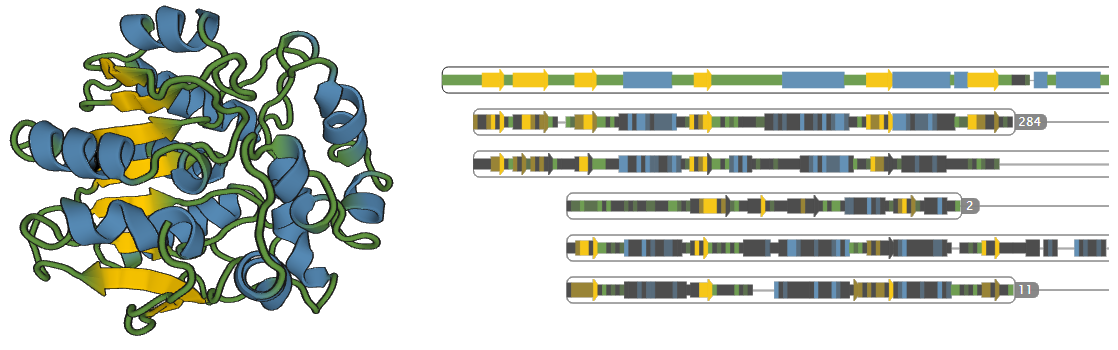
\includegraphics[width=0.9\textwidth]{pics/aquaria.png}
  \caption{Left -- cartoon representation of the DhaA haloalkane dehalogenase (PDB ID 1CQW). Right -- part of the sequential representation of DhaA along with the information about secondary structures and several other structures sequentially aligned to DhaA. Images generated using the Aquaria tool by O'Donoghue et al.~\cite{odonoghue2015}.}
  \label{fig:aquaria}
\end{figure*}

When comparing several protein structures, e.g., when searching for similar structures in order to get the information about an unknown protein, there are several existing algorithms for aligning such structures.
These algorithms are aligning the whole structures (structure alignment) or are parsing the sequence of amino acids and searching for corresponding patterns (sequence alignment). 
The results of these alignments are traditionally presented in a form of color-coded one-dimensional sequential information (see Figure~\ref{fig:align}).
Each row represents one protein structure and the user can observe the similarities and differences between protein chains by exploring the columns.
Some methods equip the sequence with the information about secondary structures (see Figure~\ref{fig:aquaria} right).
However, all of them lack the mutual spatial orientation of the secondary structures of the aligned structures.
This information is crucial in many cases, namely when exploring the protein inner void space playing a significant role in protein reactivity with other molecules.
This void space is determined by the surrounding amino acids, i.e., secondary structures. 
Therefore, the changes in the spatial position of the secondary structures directly influence the volume and shape of the void space.

\begin{figure}[th]
  \centering
  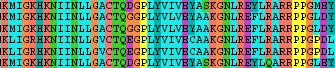
\includegraphics[width=0.9\columnwidth]{pics/align.png}
  \caption{Example of the sequence alignment visualization.}
  \label{fig:align}
\end{figure}

The mutual spatial arrangement of the secondary structures can be easily observed in a 3D view. 
However, for comparison of multiple proteins, such a representation is very limited with respect to its scalability.
In other words, due to the occlusion problems, the spatial representation is suitable for comparison of only few structures. 
Figure~\ref{fig:many} demonstrates the case when six similar proteins are aligned.
Even with such a small number of molecules it is hard to perceive the differences in the secondary structure positions.

%One of the most important ones is the presence of a void space inside the protein which directly influences the protein reactivity with a small ligand. 
%The interaction with the ligand occurs often deeply inside the protein and the 

\begin{figure}[th]
  \centering
  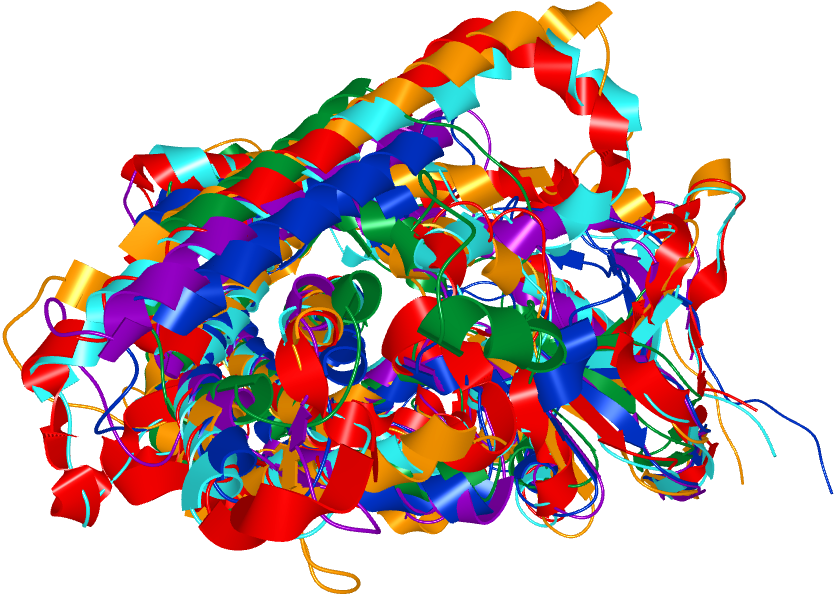
\includegraphics[width=0.9\columnwidth]{pics/many.png}
  \caption{Structure alignment of six proteins with similar structure visualized in 3D.}
  \label{fig:many}
\end{figure}

To overcome the problems of the lack of mutual arrangement of the compared protein in the sequential representation and problems with occlusion in the spatial view, we propose a new method designed to serve as a tool for comparison of multiple structures and intuitive exploration of their spatial differences.
It takes the advantages of the sequential information which consists of individual secondary structures and when comparing this sequence with other proteins, it encodes the mutual spatial arrangement of the secondary structures of the aligned proteins.
In consequence, the user can observe this arrangement without the occlusion problems of the 3D view.
Our solution also utilizes the fact that the domain experts are well accustomed with the sequential representation as well as with secondary structures and their cartoon representation. 
Therefore, our proposed visualization is interactively linked with the 3D view.
Selection of interesting secondary structures in the novel representation is directly projected to this spatial view. 

\subsection*{Related Work}

\cite{Stolte2015}, maybe also \cite{Nguyen2013}

\section*{Methodology}
Our newly proposed method bridges the gap between the one-dimensional and three-dimensional representations of the protein chain.
Moreover, it serves for fast and intuitive multiple comparison of proteins when it helps to reveal the similarities and differences between the aligned chains, namely their secondary structures.
The 3D representation is not suitable for such comparison because of the occlusion problems.
However, the spatial arrangement and mutual orientation of the aligned secondary structures highly influences the protein properties.
So it is desirable to communicate this information in the visualization.
On the other hand, the 1D sequential representation of the chain clearly communicates the protein constitution and removes the occlusion problem.
We also utilize the fact that the domain experts are well accustomed with both sequential and cartoon representations.
Therefore, we combined the qualities of both representations and proposed a novel method for comparison and interactive exploration of multiple aligned protein chains.

The input data consist of a set of proteins in the PDB format and are aligned with respect to their structure.
The alignment is performed using the Combinatorial Extension (CE) algorithm~\cite{Shindyalov1998}. 
One protein chain is selected as reference and the remaining proteins are aligned to it.
For each aligned protein this algorithm outputs the transformed positions of its atoms and the RMSD (root-mean-square deviation) number expressing the difference between the reference and aligned protein.  
The results are loaded to our newly proposed representation consisting of the following parts (see Figure~\ref{fig:design}):
\begin{itemize}
\item 3D visualization window showing all aligned proteins (it utilizes the PV viewer available in SWISS-MODEL tool~\cite{biasini2014})
\item superimposition and juxtaposition sequential representations of the secondary structures of aligned proteins
\end{itemize}

In the following we describe the design rationale behind the newly proposed sequential representation in detail.

\begin{figure*}[t!]
  \centering
  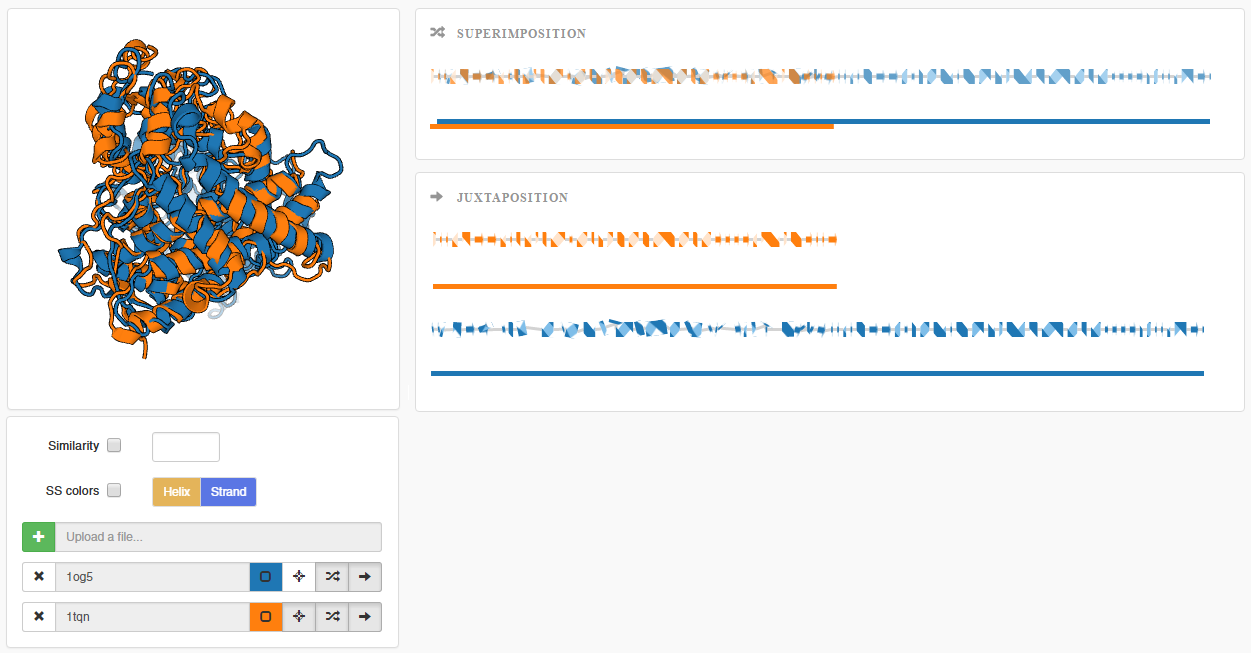
\includegraphics[height=3.5in]{pics/design.png}
  \caption{Overview of the system consisting of three main parts. TODO}
  \label{fig:design}
\end{figure*}


\subsection*{Design}
The design of the proposed sequential visualization is based on the following requirements:
\begin{itemize}
\item it should convey the information about the constitution of the protein chain wrt. its secondary structures
\item it should serve for multiple comparison of protein chains in represented by its secondary structures
\item the user should be able to easily see the similarities and differences between the chains
\item the user should have the information about the global similarity between proteins 
\item the user should be able to interact with the system in order to explore the similarities and differences in detail
\end{itemize}

Figure~\ref{fig:element} shows the basic element of our proposed visualization.
It demonstrates the case when two proteins chains are aligned.
It consists of two main parts.
The main top part represents the sequential information about protein chain along with its secondary structures.
The bottom part serves for interactive navigation through the protein chain in the top part. 
It informs the user about the length and overall alignment of the compared structures.
Moreover, it enables the user to navigate through the chain and select only an interesting part of the aligned chains which is then zoomed in the top part.

\begin{figure*}[t!]
  \centering
  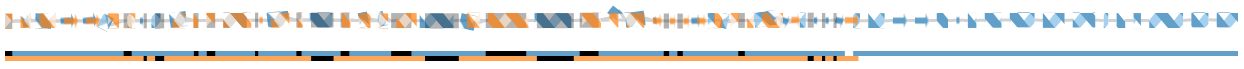
\includegraphics[width=0.9\textwidth]{pics/element.png}
  \caption{Basic element of our proposed visualization consisting of two main parts. The top part shows the secondary structures of the aligned proteins, the bottom part serves for general overview and interactive navigation and selection.}
  \label{fig:element}
\end{figure*}

%Strong points of our representation:
%\begin{itemize}
%\item interactive manipulation
%\item predefined ranking according to RMSD
%\item linking with 3D
%\item filtering (removing the most different proteins)
%\end{itemize}

\subsection*{Implementation}
%With the use of the Combinatorial Extension (CE) algorithm for structure alignment~\cite{Shindyalov1998} and force layout algorithm, we let the structures to align in 3D, so there is no deformation caused by choosing a particular projection or distortion. 
%At the end, we visualize the flattened molecules as if they were stretched out from 3D by pulling the chosen reference molecule at its ends into a straight line, so the actual length of secondary structures is preserved as well as the position of near structures of other molecules which are “locked” to the reference molecule.
%Algorithm - GAPS - Detail exploration of differences of two molecules

\subsubsection{Introduction}
We may imagine molecule that contains structures as a thread with colored beads on it. 
Each of these two threads may or may not contain complete set of beads and these beads may not be in the same order. 
Beads may be moved along the thread but their order cannot change. 
From protein structure point of view we are interested in those parts where these two threads have not the same order of their beads or some beads are missing. 
We are searching for gaps in any of these two threads/protein chains. 
Imagine that you put both threads along each other and you are moving beads along the thread such a way to achieve the same color of beads to be aligned. 
The best solution would be to minimize the amount of gaps, respectively separated beads with no pair. 
%Thus the pair making basic algorithm. 
This requires a non trivial recursive algorithm that may be very costly for memory and computational time and its description will be only pseudo-coded here. 
We will reference this algorithm as Global Best Effort and its implementation is in the stage of optimization for purposes of molecule structure matchmaking. 
Our greedy approach takes simpler approach but already has promising results with acceptable running times.

\subsubsection{The Greedy Algorithm}
The main idea of this algorithm is to find gaps. 
The input for the algorithm is formed by two molecules. 
The output contains these two molecules with added gaps. 
The algorithm uses distance search and structure comparator. 
The idea for this algorithm comes from the double stack algorithm.
The algorithm runs until both molecules are fully traversed and uses per-step approach. 
In each step a secondary structure from at least one molecule has to be added to the output. 
!!!!!!!!!!If any gap happens, the progress on input molecules will not be the same, but as algorithm progress this may change and so.

\textbf{Match Making function}
Each matchmaking from molecule A to molecule B is done only from the current index of progress on each molecule. 
The molecules are traversed from the current index to the end of molecule. 
First match is returned. 
At the moment only distance in 3D and structure type are considered in matchmaking. 
In future, penalization for number of possible gaps will be added. 
Even though this penalization is already implemented in terms of first match. 
For Global Best Effort algorithm Match making function will have to take responsibility for best match finding.

In each step the algorithm decides what to include in output molecules and how to progress on input molecules. 
Algorithm holds progress in both input molecules.

\begin{enumerate}
	\item 
	If any molecule is already processed, fill output of that molecule with gaps and fill the other molecule with structures that left. 
	This may be imagined as filling the tail.
	\item  
	Find best matches from one molecule to another and vice versa, according to the match making function earlier. 
	Take match that has minimum gaps that is needed. 
	Now molecule A will represent the structure which pair has been found in molecule B. 
	Fill the output of molecule A with gaps in ratio 1:1 to structures that will be added to output of structure B. 
	Add structure from input A to output of molecule A and same in molecule B. 
	Progress input counter in molecule A by one and in molecule B by 1 + structures added to output of molecule B.   
  \item If no match is returned from both search add gap to molecule A and structure from molecule A to output of molecule A. 
	Add structure from molecule B and gap to molecule B. 
	Progress the counter on both molecules A and B.
	\item If both molecules are at end the solution has been found.
\end{enumerate}

\subsubsection{Global Best Effort}
Motivation:
Imagine the previous nit where both of nits have the colors in this order:
 
A: RED  , BLUE , YELLOW

B: GREEN, BLUE , YELLOW, RED

There are two possibilities for output:

A: RED, GAP  , BLUE, YELLOW, GAP

B: GAP, GREEN, BLUE, YELLOW, RED

or

A: GAP  , GAP , GAP   , RED, BLUE, YELLOW

B: GREEN, BLUE, YELLOW, RED, GAP , GAP   

From the point of nit it is simple. 
The first option of nit it is easy. 
The first option will by found. 
In 3D match making situation may not be the same. 
Imagine the RED structures are very close to each other. 
The RED in molecule A is very close to RED in molecule B. 
The matchmaking function will definitely found out that the RED structures are the best match and found out that GREEN has no match in molecule A.
From this point the second solution will be taken even if it is not the best estimation in global scale.

Solution:
Algorithm already uses recursive calling.
It is derived from your Hunger algorithm.
Imagine it as a tree that is build depth first with early cut, so dead end computation with already big penalization are cut before additional computation.
Algorithm stores all solutions in solutions pool.
 
\begin{enumerate}
	\item 
	If penalisation of solution is already too big.
	Stop this branch and do not continue.
	\item 
	If tail of any molecule happens do as hunger algorithm
  \item 
	Instead of computing only first match from each molecule, compute all matches.
	This may sound very demanding but it is required. 
	Do not forget that Match Making function takes distance as a main parameter for match search, thus the possible pairs may be greatly minimised.
	\item
	For each of possible match do operation as would hunger algorithm and continue.
	This is done via recursion and penalization for amount of gap is passed with each call of function.
  \item 
  If no match is found continue as a hunger algorithm.
  \item 
  If both molecules are at end continue as a hunger algorithm.
\end{enumerate}
As the algorithm computes depth first solutions are found. Steps 2 and 6 adding solutions to solution pool. The solution pool has to be filtered from time to time. At first solutions with higher penalisation will be added to pool, because the maximum penalisation will not be set. As solutions will be added to pool maximum penalisation will be set to lowest from the pool. In each solution push to pool all solutions in pool with solution higher penalisation than minimal penalistion will be removed from pool. By this only solutions with lowes penalisation will stay in pool.

\subsubsection{Dynamics}
Typically in dynamics we are comparing more than two molecules at same time. 
As seen earlier, Hunger and Best Effort algorithm modifies the output molecules. 
This is not acceptable in global scale as we may have to compare each molecule with each molecule and there is not a molecule that can not change. 
Another approach is required. 
As we only comparing same molecule in different time we are sure that structures will not change positions, even if they may be missing respectively not recognised in that time moment. Algorithm goes through all molecule time snapshots at each time. Algorithm takes all snapshots and returns one super snapshot without gaps but with all structures in order from beginning found in all snapshots. Algorithm holds position for each molecule snapshot.

If molecules are fully traversed end the solution.
For each snapshot (snapshot A):
Take current structure (structure A) and found that structure on each other snapshot (snapshot X). Traverse only nodes that are has not been already passed on traversed each structure (snapshot X). 
If GAP would be required. Do not search further and take another snapshot to take structure to find. Note that that in reality match will be found usually within 5 steps on chain so it is very rare to traverse whole molecule. (Time reduction)
If structures is found that do not require GAP (structure is missing in other snapshots or it is in first position to take) put it into an output super snapshot and progress on each structure where the structure has been found.
If for all snapshots GAP would be required to put (each snapshot would have to produce different structure on same position ... very unexpected ... maybe even impossible) take all snapshots and put all stuctures into super snapshot and update counter on each snapshot.

When this part of algorithm is ended. Run Hunger Algorithm with updated Match Making function. Match Making function will only take in count the structure type and not distance. From the experience we presume that the distance of the structures will not change that much to count with it. There is no need for Best Effort algorithm because the snapshots will be compared with super snapshot that has to encapsulate all snapshots. The super snapshot will no change so input of super snapshot will be the same as output for super snapshot from Hunger algorithm. 

On the final visuallisation gaps represent where are the dynamics points of interest. If no gaps are found the threshold for structure recognision may be too big and if many gaps are found the molecule may be instable or the threshold is set very strictly.
 

\subsection*{Interaction}

The 3D view and 2D view are both interactive -- basic information about the secondary structure is shown when mouse is moving over the visualizations and a structure is highlighted in green when a structure is selected by a mouse click. Moreover, the 3D and 2D views are interconnected, thus creating a unique way to explore the molecules -- when any of the structure is clicked on, the highlight is visible immediately in both views. This feature gives the user very important context of the actual spatial positions of the selected structures and enables him or her to interact with both views independtly, yet still in context. Therefore, the user does not have to tediously decode the flattened visualization trying to figure out what the spatial context of a given structure is, he or she just has to glipms into the 3D view and then continue to the next interesting area for exploration.

The visibility of molecules and their attributes in both views is possible via buttons in configuration panel below the 3D viewer. Molecules in the juxtaposition view are sortable, so the user can see the differences between the pairs of molecules of his or her choice.

%\begin{figure*}[t!]
%  \centering
%  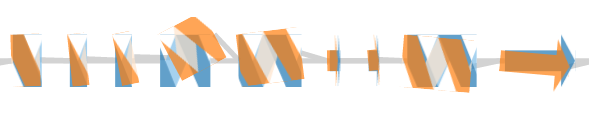
\includegraphics[height=3.5in]{pics/teaser.png}
%  \caption{Example two-column figure. To insert a single column figure, remove the * in the two figure tags. }
%  \label{fig:interface}
%\end{figure*}


\section*{Results and Discussion}
TODO

\subsection*{Case Study}

\section*{Conclusions}
TODO

Future work
- algorithm for generating gaps -- design and implement non-trivial approach to visualizing gaps in superimposition of more than two structures
- introduce a similarity index which would be created with the cooperation of domain experts
- automatic suggestions of interesting parts of the aligned chains -- and highlight them in both 2D and 3D
- contour based visualization of many superimposed structures
- encode additional information into the visualization, e.g. tunnels, ligands (see what is already done in STAR)
%%%%%%%%%%%%%%%%%%%%%%%%%%%%%%%%%%%%%%%%%%%%%% 
%%                                          %%
%% Backmatter begins here                   %%
%%                                          %%
%%%%%%%%%%%%%%%%%%%%%%%%%%%%%%%%%%%%%%%%%%%%%%

\begin{backmatter}

%\section*{List of abbreviations used}
%TIM: \textit{triosephosphate isomerase}, scTIM: \textit{saccharomyces
%cerevisiae triosephosphate isomerase}, dTIM: \textit{defective triosephosphate
%isomerase}, PDB: \textit{protein data bank}.

\section*{Competing interests}
The authors declare that they have no competing interests.


%%%%%%%%%%%%%%%%%%%%%%%%%%%%%%%%%%%%%%%%%%%%%%%%%%%%%%%%%%%%%
%%                  The Bibliography                       %%
%%                                                         %%
%%  Bmc_mathpys.bst  will be used to                       %%
%%  create a .BBL file for submission.                     %%
%%  After submission of the .TEX file,                     %%
%%  you will be prompted to submit your .BBL file.         %%
%%                                                         %%
%%                                                         %%
%%  Note that the displayed Bibliography will not          %%
%%  necessarily be rendered by Latex exactly as specified  %%
%%  in the online Instructions for Authors.                %%
%%                                                         %%
%%%%%%%%%%%%%%%%%%%%%%%%%%%%%%%%%%%%%%%%%%%%%%%%%%%%%%%%%%%%%

% if your bibliography is in bibtex format, use those commands:
\bibliographystyle{bmc-mathphys} % Style BST file
\bibliography{bmc_article}      % Bibliography file (usually '*.bib' )

% or include bibliography directly:
% \begin{thebibliography}
% \bibitem{b1}
% \end{thebibliography}

%%%%%%%%%%%%%%%%%%%%%%%%%%%%%%%%%%%
%%                               %%
%% Figures                       %%
%%                               %%
%% NB: this is for captions and  %%
%% Titles. All graphics must be  %%
%% submitted separately and NOT  %%
%% included in the Tex document  %%
%%                               %%
%%%%%%%%%%%%%%%%%%%%%%%%%%%%%%%%%%%

%%
%% Do not use \listoffigures as most will included as separate files

%\section*{Figures}
%  \begin{figure}[h!]
 % \caption{\csentence{Sample figure title.}
  %    A short description of the figure content
   %   should go here.}
   %   \end{figure}

%\begin{figure}[h!]
 % \caption{\csentence{Sample figure title.}
  %    Figure legend text.}
  %    \end{figure}

%%%%%%%%%%%%%%%%%%%%%%%%%%%%%%%%%%%
%%                               %%
%% Tables                        %%
%%                               %%
%%%%%%%%%%%%%%%%%%%%%%%%%%%%%%%%%%%

%% Use of \listoftables is discouraged.
%%
%\section*{Tables}
%\begin{table}[h!]
%\caption{Sample table title. This is where the description of the table should go.}
 %     \begin{tabular}{cccc}
%        \hline
 %          & B1  &B2   & B3\\ \hline
 %       A1 & 0.1 & 0.2 & 0.3\\
 %       A2 & ... & ..  & .\\
 %       A3 & ..  & .   & .\\ \hline
 %     \end{tabular}
%\end{table}

%%%%%%%%%%%%%%%%%%%%%%%%%%%%%%%%%%%
%%                               %%
%% Additional Files              %%
%%                               %%
%%%%%%%%%%%%%%%%%%%%%%%%%%%%%%%%%%%

%\section*{Additional Files}
%  \subsection*{Additional file 1 --- Sample additional file title}
%    Additional file descriptions text (including details of how to
%    view the file, if it is in a non-standard format or the file extension).  This might
%    refer to a multi-page table or a figure.

%  \subsection*{Additional file 2 --- Sample additional file title}
%    Additional file descriptions text.

\end{backmatter}
\end{document}
